% CVPR 2022 Paper Template
% based on the CVPR template provided by Ming-Ming Cheng (https://github.com/MCG-NKU/CVPR_Template)
% modified and extended by Stefan Roth (stefan.roth@NOSPAMtu-darmstadt.de)

\documentclass[10pt,twocolumn,letterpaper]{article}

%%%%%%%%% PAPER TYPE  - PLEASE UPDATE FOR FINAL VERSION
\usepackage[review]{cvpr}      % To produce the REVIEW version
%\usepackage{cvpr}              % To produce the CAMERA-READY version
%\usepackage[pagenumbers]{cvpr} % To force page numbers, e.g. for an arXiv version

% Include other packages here, before hyperref.
\usepackage{graphicx}
\usepackage{amsmath}
\usepackage{amssymb}
\usepackage{booktabs}

\usepackage{microtype}
\usepackage{xcolor}
\newcommand{\oo}[1]{\textcolor{orange}{#1}}
%%%%% NEW MATH DEFINITIONS %%%%%

\usepackage{amsmath,amsfonts,bm}

% Mark sections of captions for referring to divisions of figures
\newcommand{\figleft}{{\em (Left)}}
\newcommand{\figcenter}{{\em (Center)}}
\newcommand{\figright}{{\em (Right)}}
\newcommand{\figtop}{{\em (Top)}}
\newcommand{\figbottom}{{\em (Bottom)}}
\newcommand{\captiona}{{\em (a)}}
\newcommand{\captionb}{{\em (b)}}
\newcommand{\captionc}{{\em (c)}}
\newcommand{\captiond}{{\em (d)}}

% Highlight a newly defined term
\newcommand{\newterm}[1]{{\bf #1}}


% Figure reference, lower-case.
\def\figref#1{figure~\ref{#1}}
% Figure reference, capital. For start of sentence
\def\Figref#1{Figure~\ref{#1}}
\def\twofigref#1#2{figures \ref{#1} and \ref{#2}}
\def\quadfigref#1#2#3#4{figures \ref{#1}, \ref{#2}, \ref{#3} and \ref{#4}}
% Section reference, lower-case.
\def\secref#1{section~\ref{#1}}
% Section reference, capital.
\def\Secref#1{Section~\ref{#1}}
% Reference to two sections.
\def\twosecrefs#1#2{sections \ref{#1} and \ref{#2}}
% Reference to three sections.
\def\secrefs#1#2#3{sections \ref{#1}, \ref{#2} and \ref{#3}}
% Reference to an equation, lower-case.
\def\eqref#1{equation~\ref{#1}}
% Reference to an equation, upper case
\def\Eqref#1{Equation~\ref{#1}}
% A raw reference to an equation---avoid using if possible
\def\plaineqref#1{\ref{#1}}
% Reference to a chapter, lower-case.
\def\chapref#1{chapter~\ref{#1}}
% Reference to an equation, upper case.
\def\Chapref#1{Chapter~\ref{#1}}
% Reference to a range of chapters
\def\rangechapref#1#2{chapters\ref{#1}--\ref{#2}}
% Reference to an algorithm, lower-case.
\def\algref#1{algorithm~\ref{#1}}
% Reference to an algorithm, upper case.
\def\Algref#1{Algorithm~\ref{#1}}
\def\twoalgref#1#2{algorithms \ref{#1} and \ref{#2}}
\def\Twoalgref#1#2{Algorithms \ref{#1} and \ref{#2}}
% Reference to a part, lower case
\def\partref#1{part~\ref{#1}}
% Reference to a part, upper case
\def\Partref#1{Part~\ref{#1}}
\def\twopartref#1#2{parts \ref{#1} and \ref{#2}}

\def\ceil#1{\lceil #1 \rceil}
\def\floor#1{\lfloor #1 \rfloor}
\def\1{\bm{1}}
\newcommand{\train}{\mathcal{D}}
\newcommand{\valid}{\mathcal{D_{\mathrm{valid}}}}
\newcommand{\test}{\mathcal{D_{\mathrm{test}}}}

\def\eps{{\epsilon}}


% Random variables
\def\reta{{\textnormal{$\eta$}}}
\def\ra{{\textnormal{a}}}
\def\rb{{\textnormal{b}}}
\def\rc{{\textnormal{c}}}
\def\rd{{\textnormal{d}}}
\def\re{{\textnormal{e}}}
\def\rf{{\textnormal{f}}}
\def\rg{{\textnormal{g}}}
\def\rh{{\textnormal{h}}}
\def\ri{{\textnormal{i}}}
\def\rj{{\textnormal{j}}}
\def\rk{{\textnormal{k}}}
\def\rl{{\textnormal{l}}}
% rm is already a command, just don't name any random variables m
\def\rn{{\textnormal{n}}}
\def\ro{{\textnormal{o}}}
\def\rp{{\textnormal{p}}}
\def\rq{{\textnormal{q}}}
\def\rr{{\textnormal{r}}}
\def\rs{{\textnormal{s}}}
\def\rt{{\textnormal{t}}}
\def\ru{{\textnormal{u}}}
\def\rv{{\textnormal{v}}}
\def\rw{{\textnormal{w}}}
\def\rx{{\textnormal{x}}}
\def\ry{{\textnormal{y}}}
\def\rz{{\textnormal{z}}}

% Random vectors
\def\rvepsilon{{\mathbf{\epsilon}}}
\def\rvtheta{{\mathbf{\theta}}}
\def\rva{{\mathbf{a}}}
\def\rvb{{\mathbf{b}}}
\def\rvc{{\mathbf{c}}}
\def\rvd{{\mathbf{d}}}
\def\rve{{\mathbf{e}}}
\def\rvf{{\mathbf{f}}}
\def\rvg{{\mathbf{g}}}
\def\rvh{{\mathbf{h}}}
\def\rvu{{\mathbf{i}}}
\def\rvj{{\mathbf{j}}}
\def\rvk{{\mathbf{k}}}
\def\rvl{{\mathbf{l}}}
\def\rvm{{\mathbf{m}}}
\def\rvn{{\mathbf{n}}}
\def\rvo{{\mathbf{o}}}
\def\rvp{{\mathbf{p}}}
\def\rvq{{\mathbf{q}}}
\def\rvr{{\mathbf{r}}}
\def\rvs{{\mathbf{s}}}
\def\rvt{{\mathbf{t}}}
\def\rvu{{\mathbf{u}}}
\def\rvv{{\mathbf{v}}}
\def\rvw{{\mathbf{w}}}
\def\rvx{{\mathbf{x}}}
\def\rvy{{\mathbf{y}}}
\def\rvz{{\mathbf{z}}}

% Elements of random vectors
\def\erva{{\textnormal{a}}}
\def\ervb{{\textnormal{b}}}
\def\ervc{{\textnormal{c}}}
\def\ervd{{\textnormal{d}}}
\def\erve{{\textnormal{e}}}
\def\ervf{{\textnormal{f}}}
\def\ervg{{\textnormal{g}}}
\def\ervh{{\textnormal{h}}}
\def\ervi{{\textnormal{i}}}
\def\ervj{{\textnormal{j}}}
\def\ervk{{\textnormal{k}}}
\def\ervl{{\textnormal{l}}}
\def\ervm{{\textnormal{m}}}
\def\ervn{{\textnormal{n}}}
\def\ervo{{\textnormal{o}}}
\def\ervp{{\textnormal{p}}}
\def\ervq{{\textnormal{q}}}
\def\ervr{{\textnormal{r}}}
\def\ervs{{\textnormal{s}}}
\def\ervt{{\textnormal{t}}}
\def\ervu{{\textnormal{u}}}
\def\ervv{{\textnormal{v}}}
\def\ervw{{\textnormal{w}}}
\def\ervx{{\textnormal{x}}}
\def\ervy{{\textnormal{y}}}
\def\ervz{{\textnormal{z}}}

% Random matrices
\def\rmA{{\mathbf{A}}}
\def\rmB{{\mathbf{B}}}
\def\rmC{{\mathbf{C}}}
\def\rmD{{\mathbf{D}}}
\def\rmE{{\mathbf{E}}}
\def\rmF{{\mathbf{F}}}
\def\rmG{{\mathbf{G}}}
\def\rmH{{\mathbf{H}}}
\def\rmI{{\mathbf{I}}}
\def\rmJ{{\mathbf{J}}}
\def\rmK{{\mathbf{K}}}
\def\rmL{{\mathbf{L}}}
\def\rmM{{\mathbf{M}}}
\def\rmN{{\mathbf{N}}}
\def\rmO{{\mathbf{O}}}
\def\rmP{{\mathbf{P}}}
\def\rmQ{{\mathbf{Q}}}
\def\rmR{{\mathbf{R}}}
\def\rmS{{\mathbf{S}}}
\def\rmT{{\mathbf{T}}}
\def\rmU{{\mathbf{U}}}
\def\rmV{{\mathbf{V}}}
\def\rmW{{\mathbf{W}}}
\def\rmX{{\mathbf{X}}}
\def\rmY{{\mathbf{Y}}}
\def\rmZ{{\mathbf{Z}}}

% Elements of random matrices
\def\ermA{{\textnormal{A}}}
\def\ermB{{\textnormal{B}}}
\def\ermC{{\textnormal{C}}}
\def\ermD{{\textnormal{D}}}
\def\ermE{{\textnormal{E}}}
\def\ermF{{\textnormal{F}}}
\def\ermG{{\textnormal{G}}}
\def\ermH{{\textnormal{H}}}
\def\ermI{{\textnormal{I}}}
\def\ermJ{{\textnormal{J}}}
\def\ermK{{\textnormal{K}}}
\def\ermL{{\textnormal{L}}}
\def\ermM{{\textnormal{M}}}
\def\ermN{{\textnormal{N}}}
\def\ermO{{\textnormal{O}}}
\def\ermP{{\textnormal{P}}}
\def\ermQ{{\textnormal{Q}}}
\def\ermR{{\textnormal{R}}}
\def\ermS{{\textnormal{S}}}
\def\ermT{{\textnormal{T}}}
\def\ermU{{\textnormal{U}}}
\def\ermV{{\textnormal{V}}}
\def\ermW{{\textnormal{W}}}
\def\ermX{{\textnormal{X}}}
\def\ermY{{\textnormal{Y}}}
\def\ermZ{{\textnormal{Z}}}

% Vectors
\def\vzero{{\bm{0}}}
\def\vone{{\bm{1}}}
\def\vmu{{\bm{\mu}}}
\def\vtheta{{\bm{\theta}}}
\def\va{{\bm{a}}}
\def\vb{{\bm{b}}}
\def\vc{{\bm{c}}}
\def\vd{{\bm{d}}}
\def\ve{{\bm{e}}}
\def\vf{{\bm{f}}}
\def\vg{{\bm{g}}}
\def\vh{{\bm{h}}}
\def\vi{{\bm{i}}}
\def\vj{{\bm{j}}}
\def\vk{{\bm{k}}}
\def\vl{{\bm{l}}}
\def\vm{{\bm{m}}}
\def\vn{{\bm{n}}}
\def\vo{{\bm{o}}}
\def\vp{{\bm{p}}}
\def\vq{{\bm{q}}}
\def\vr{{\bm{r}}}
\def\vs{{\bm{s}}}
\def\vt{{\bm{t}}}
\def\vu{{\bm{u}}}
\def\vv{{\bm{v}}}
\def\vw{{\bm{w}}}
\def\vx{{\bm{x}}}
\def\vy{{\bm{y}}}
\def\vz{{\bm{z}}}

% Elements of vectors
\def\evalpha{{\alpha}}
\def\evbeta{{\beta}}
\def\evepsilon{{\epsilon}}
\def\evlambda{{\lambda}}
\def\evomega{{\omega}}
\def\evmu{{\mu}}
\def\evpsi{{\psi}}
\def\evsigma{{\sigma}}
\def\evtheta{{\theta}}
\def\eva{{a}}
\def\evb{{b}}
\def\evc{{c}}
\def\evd{{d}}
\def\eve{{e}}
\def\evf{{f}}
\def\evg{{g}}
\def\evh{{h}}
\def\evi{{i}}
\def\evj{{j}}
\def\evk{{k}}
\def\evl{{l}}
\def\evm{{m}}
\def\evn{{n}}
\def\evo{{o}}
\def\evp{{p}}
\def\evq{{q}}
\def\evr{{r}}
\def\evs{{s}}
\def\evt{{t}}
\def\evu{{u}}
\def\evv{{v}}
\def\evw{{w}}
\def\evx{{x}}
\def\evy{{y}}
\def\evz{{z}}

% Matrix
\def\mA{{\bm{A}}}
\def\mB{{\bm{B}}}
\def\mC{{\bm{C}}}
\def\mD{{\bm{D}}}
\def\mE{{\bm{E}}}
\def\mF{{\bm{F}}}
\def\mG{{\bm{G}}}
\def\mH{{\bm{H}}}
\def\mI{{\bm{I}}}
\def\mJ{{\bm{J}}}
\def\mK{{\bm{K}}}
\def\mL{{\bm{L}}}
\def\mM{{\bm{M}}}
\def\mN{{\bm{N}}}
\def\mO{{\bm{O}}}
\def\mP{{\bm{P}}}
\def\mQ{{\bm{Q}}}
\def\mR{{\bm{R}}}
\def\mS{{\bm{S}}}
\def\mT{{\bm{T}}}
\def\mU{{\bm{U}}}
\def\mV{{\bm{V}}}
\def\mW{{\bm{W}}}
\def\mX{{\bm{X}}}
\def\mY{{\bm{Y}}}
\def\mZ{{\bm{Z}}}
\def\mBeta{{\bm{\beta}}}
\def\mPhi{{\bm{\Phi}}}
\def\mLambda{{\bm{\Lambda}}}
\def\mSigma{{\bm{\Sigma}}}

% Tensor
\DeclareMathAlphabet{\mathsfit}{\encodingdefault}{\sfdefault}{m}{sl}
\SetMathAlphabet{\mathsfit}{bold}{\encodingdefault}{\sfdefault}{bx}{n}
\newcommand{\tens}[1]{\bm{\mathsfit{#1}}}
\def\tA{{\tens{A}}}
\def\tB{{\tens{B}}}
\def\tC{{\tens{C}}}
\def\tD{{\tens{D}}}
\def\tE{{\tens{E}}}
\def\tF{{\tens{F}}}
\def\tG{{\tens{G}}}
\def\tH{{\tens{H}}}
\def\tI{{\tens{I}}}
\def\tJ{{\tens{J}}}
\def\tK{{\tens{K}}}
\def\tL{{\tens{L}}}
\def\tM{{\tens{M}}}
\def\tN{{\tens{N}}}
\def\tO{{\tens{O}}}
\def\tP{{\tens{P}}}
\def\tQ{{\tens{Q}}}
\def\tR{{\tens{R}}}
\def\tS{{\tens{S}}}
\def\tT{{\tens{T}}}
\def\tU{{\tens{U}}}
\def\tV{{\tens{V}}}
\def\tW{{\tens{W}}}
\def\tX{{\tens{X}}}
\def\tY{{\tens{Y}}}
\def\tZ{{\tens{Z}}}


% Graph
\def\gA{{\mathcal{A}}}
\def\gB{{\mathcal{B}}}
\def\gC{{\mathcal{C}}}
\def\gD{{\mathcal{D}}}
\def\gE{{\mathcal{E}}}
\def\gF{{\mathcal{F}}}
\def\gG{{\mathcal{G}}}
\def\gH{{\mathcal{H}}}
\def\gI{{\mathcal{I}}}
\def\gJ{{\mathcal{J}}}
\def\gK{{\mathcal{K}}}
\def\gL{{\mathcal{L}}}
\def\gM{{\mathcal{M}}}
\def\gN{{\mathcal{N}}}
\def\gO{{\mathcal{O}}}
\def\gP{{\mathcal{P}}}
\def\gQ{{\mathcal{Q}}}
\def\gR{{\mathcal{R}}}
\def\gS{{\mathcal{S}}}
\def\gT{{\mathcal{T}}}
\def\gU{{\mathcal{U}}}
\def\gV{{\mathcal{V}}}
\def\gW{{\mathcal{W}}}
\def\gX{{\mathcal{X}}}
\def\gY{{\mathcal{Y}}}
\def\gZ{{\mathcal{Z}}}

% Sets
\def\sA{{\mathbb{A}}}
\def\sB{{\mathbb{B}}}
\def\sC{{\mathbb{C}}}
\def\sD{{\mathbb{D}}}
% Don't use a set called E, because this would be the same as our symbol
% for expectation.
\def\sF{{\mathbb{F}}}
\def\sG{{\mathbb{G}}}
\def\sH{{\mathbb{H}}}
\def\sI{{\mathbb{I}}}
\def\sJ{{\mathbb{J}}}
\def\sK{{\mathbb{K}}}
\def\sL{{\mathbb{L}}}
\def\sM{{\mathbb{M}}}
\def\sN{{\mathbb{N}}}
\def\sO{{\mathbb{O}}}
\def\sP{{\mathbb{P}}}
\def\sQ{{\mathbb{Q}}}
\def\sR{{\mathbb{R}}}
\def\sS{{\mathbb{S}}}
\def\sT{{\mathbb{T}}}
\def\sU{{\mathbb{U}}}
\def\sV{{\mathbb{V}}}
\def\sW{{\mathbb{W}}}
\def\sX{{\mathbb{X}}}
\def\sY{{\mathbb{Y}}}
\def\sZ{{\mathbb{Z}}}

% Entries of a matrix
\def\emLambda{{\Lambda}}
\def\emA{{A}}
\def\emB{{B}}
\def\emC{{C}}
\def\emD{{D}}
\def\emE{{E}}
\def\emF{{F}}
\def\emG{{G}}
\def\emH{{H}}
\def\emI{{I}}
\def\emJ{{J}}
\def\emK{{K}}
\def\emL{{L}}
\def\emM{{M}}
\def\emN{{N}}
\def\emO{{O}}
\def\emP{{P}}
\def\emQ{{Q}}
\def\emR{{R}}
\def\emS{{S}}
\def\emT{{T}}
\def\emU{{U}}
\def\emV{{V}}
\def\emW{{W}}
\def\emX{{X}}
\def\emY{{Y}}
\def\emZ{{Z}}
\def\emSigma{{\Sigma}}

% entries of a tensor
% Same font as tensor, without \bm wrapper
\newcommand{\etens}[1]{\mathsfit{#1}}
\def\etLambda{{\etens{\Lambda}}}
\def\etA{{\etens{A}}}
\def\etB{{\etens{B}}}
\def\etC{{\etens{C}}}
\def\etD{{\etens{D}}}
\def\etE{{\etens{E}}}
\def\etF{{\etens{F}}}
\def\etG{{\etens{G}}}
\def\etH{{\etens{H}}}
\def\etI{{\etens{I}}}
\def\etJ{{\etens{J}}}
\def\etK{{\etens{K}}}
\def\etL{{\etens{L}}}
\def\etM{{\etens{M}}}
\def\etN{{\etens{N}}}
\def\etO{{\etens{O}}}
\def\etP{{\etens{P}}}
\def\etQ{{\etens{Q}}}
\def\etR{{\etens{R}}}
\def\etS{{\etens{S}}}
\def\etT{{\etens{T}}}
\def\etU{{\etens{U}}}
\def\etV{{\etens{V}}}
\def\etW{{\etens{W}}}
\def\etX{{\etens{X}}}
\def\etY{{\etens{Y}}}
\def\etZ{{\etens{Z}}}

% The true underlying data generating distribution
\newcommand{\pdata}{p_{\rm{data}}}
% The empirical distribution defined by the training set
\newcommand{\ptrain}{\hat{p}_{\rm{data}}}
\newcommand{\Ptrain}{\hat{P}_{\rm{data}}}
% The model distribution
\newcommand{\pmodel}{p_{\rm{model}}}
\newcommand{\Pmodel}{P_{\rm{model}}}
\newcommand{\ptildemodel}{\tilde{p}_{\rm{model}}}
% Stochastic autoencoder distributions
\newcommand{\pencode}{p_{\rm{encoder}}}
\newcommand{\pdecode}{p_{\rm{decoder}}}
\newcommand{\precons}{p_{\rm{reconstruct}}}

\newcommand{\laplace}{\mathrm{Laplace}} % Laplace distribution

\newcommand{\E}{\mathbb{E}}
\newcommand{\Ls}{\mathcal{L}}
\newcommand{\R}{\mathbb{R}}
\newcommand{\emp}{\tilde{p}}
\newcommand{\lr}{\alpha}
\newcommand{\reg}{\lambda}
\newcommand{\rect}{\mathrm{rectifier}}
\newcommand{\softmax}{\mathrm{softmax}}
\newcommand{\sigmoid}{\sigma}
\newcommand{\softplus}{\zeta}
\newcommand{\KL}{D_{\mathrm{KL}}}
\newcommand{\Var}{\mathrm{Var}}
\newcommand{\standarderror}{\mathrm{SE}}
\newcommand{\Cov}{\mathrm{Cov}}
% Wolfram Mathworld says $L^2$ is for function spaces and $\ell^2$ is for vectors
% But then they seem to use $L^2$ for vectors throughout the site, and so does
% wikipedia.
\newcommand{\normlzero}{L^0}
\newcommand{\normlone}{L^1}
\newcommand{\normltwo}{L^2}
\newcommand{\normlp}{L^p}
\newcommand{\normmax}{L^\infty}

\newcommand{\parents}{Pa} % See usage in notation.tex. Chosen to match Daphne's book.

\DeclareMathOperator*{\argmax}{arg\,max}
\DeclareMathOperator*{\argmin}{arg\,min}

\DeclareMathOperator{\sign}{sign}
\DeclareMathOperator{\Tr}{Tr}
\let\ab\allowbreak

\usepackage{pifont}
\newcommand{\cmark}{\ding{51}}
\newcommand{\xmark}{\ding{55}}
\usepackage{enumitem}
\usepackage{multirow}
\newcommand{\uline}[1]{\underline{#1}}

%\DeclareMathOperator*{\argmax}{arg\,max}
%\DeclareMathOperator*{\argmin}{arg\,min}

% It is strongly recommended to use hyperref, especially for the review version.
% hyperref with option pagebackref eases the reviewers' job.
% Please disable hyperref *only* if you encounter grave issues, e.g. with the
% file validation for the camera-ready version.
%
% If you comment hyperref and then uncomment it, you should delete
% ReviewTempalte.aux before re-running LaTeX.
% (Or just hit 'q' on the first LaTeX run, let it finish, and you
%  should be clear).
\usepackage[pagebackref,breaklinks,colorlinks]{hyperref}


% Support for easy cross-referencing
\usepackage[capitalize]{cleveref}
\crefname{section}{Sec.}{Secs.}
\Crefname{section}{Section}{Sections}
\Crefname{table}{Table}{Tables}
\crefname{table}{Tab.}{Tabs.}


%%%%%%%%% PAPER ID  - PLEASE UPDATE
\def\cvprPaperID{201} % *** Enter the CVPR Paper ID here
\def\confName{CVPR}
\def\confYear{2022}


\begin{document}

%%%%%%%%% TITLE - PLEASE UPDATE
\title{Enhancing Adversarial Robustness for Deep Metric Learning}

\author{Mo Zhou ~~~~~~~ Vishal Patel\\
Johns Hopkins University\\
{\tt\small mzhou32@jhu.edu ~~ vpatel36@jhu.edu}
% For a paper whose authors are all at the same institution,
% omit the following lines up until the closing ``}''.
% Additional authors and addresses can be added with ``\and'',
% just like the second author.
% To save space, use either the email address or home page, not both
}
\maketitle

%%%%%%%%% ABSTRACT
\begin{abstract}
	% background
	Deep metric learning, being vulnerable to adversarial
	attacks, has safety and security implications in its applications.
	% 
	Owing to the significance of this issue, a series of defense methods
	are proposed to improve its adversarial robustness.
	% insight
	However, as a model with triplet loss is prone to collapse with
	excessively hard samples, the existing methods refrain from using the
	classical min-max adversarial training paradigm, and hence suffer from
	inefficient learning from a strong adversary.
	% our finding
	In this paper, we reveal a significant impact of triplet sampling strategy
	on the adversarial training.
	% solution 1
	Based on this, Hardness Manipulation is proposed to adversarially perturb
	a given triplet into a specified hardness level in min-max adversarial
	training, instead of creating hardest triplets rendering model collapse.
	% solution 2
	To further improve the model performance, we propose a Gradual
	Adversary to dynamicly change the hardness level to balance metric
	learning and adversarial learning.
	% Experiment
	The proposed method is validated on three commonly
	used deep metric learning datasets, namely CUB-200-2011, Cars-196,
	and Stanford Online Product.
	% Conclusion
	Comprehensive experimental results show our method outperforms
	the existing defense methods, while achieving clearly higher
	efficiency at a lower training cost.
\end{abstract}

%%%%%%%%% BODY TEXT
\section{Introduction}
\label{sec:1}

% background and insight.

Given a set of data points, a metric gives a distance value between each pair
of them.
%
Deep Metric Learning (DML) aims to learn such a metric between two inputs (\eg,
images) leveraging the representational power of deep neural networks.
%
DML has been extensively studied~\cite{revisiting}, and has a
wide range of applications such
as image retrieval~\cite{imagesim2} and face recognition~\cite{facenet,domainface}.
%
Despite the improvements of this field thanks to the advancement of deep neural
networks, recent research works suggest that DML models are vulnerable to
adversarial attacks, where an imperceptible perturbation could incur unexpected
or covertly manipulated results~\cite{advrank,advorder}.
%
Such vulnerability poses safety, security, and fairness concerns in the
applications of DML.
%
For example, impersonation or recognition evation are possible for DML-based
face-identification system.
%
To counter the attacks (or reducing the vulnerability), it is important to
design defense methods to improve the adversarial robustness of DML models.

\begin{figure}[t]
	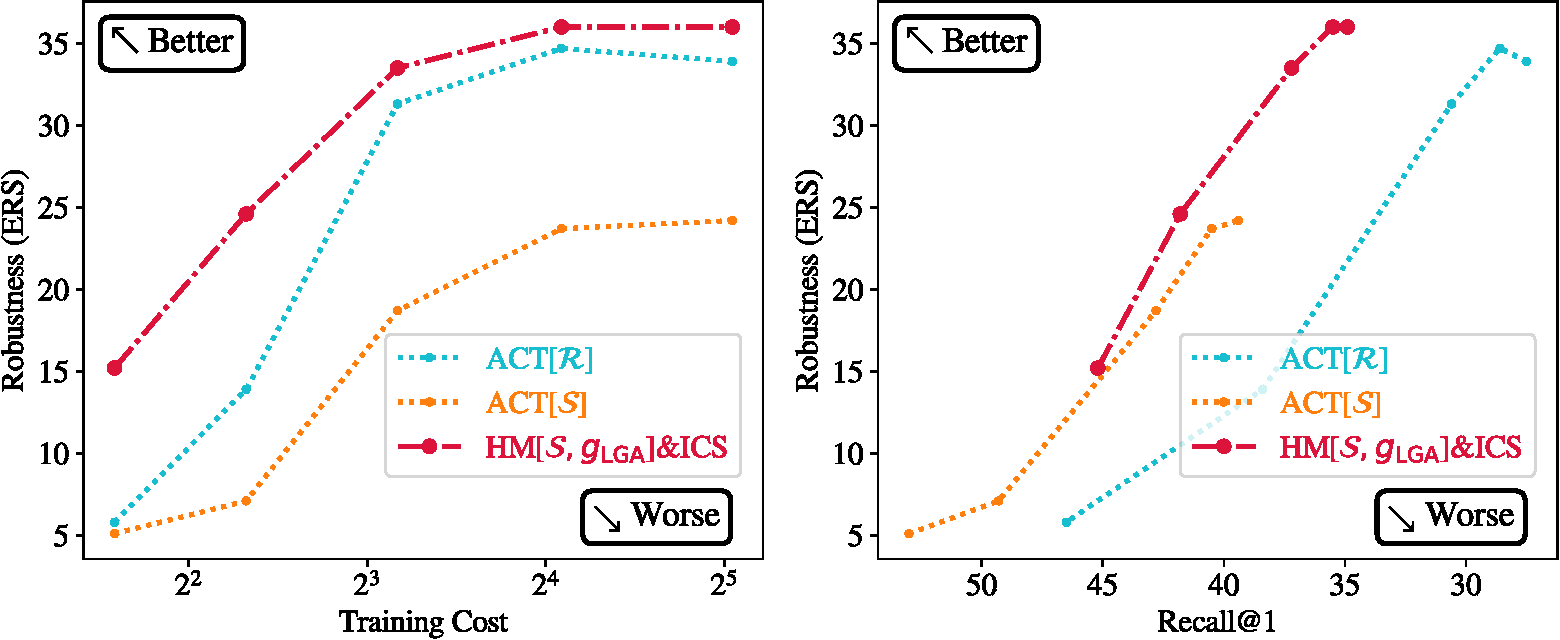
\includegraphics[width=1.0\columnwidth]{introplot.pdf}
	\caption{\oo{Performance plot with aligned conditions.
	(1) robustness and r1 under the same training cost;
	(2) r1 and training cost for reaching similar robustness;
	(3) training cost and robustness for reaching similar r1.}}
\end{figure}

% existing methods & problem
Several defense methods for DML are proposed in the
literature~\cite{advrank,robrank}, inspired by the Madry's adversarial training
method~\cite{madry}, as it is kown as one of the most effective defense methods
for deep neural network classifiers.
%
However, it has been noted that
%
(1) the robustness level achieved by the existing methods is still insufficient
to counter the attacks;
%
(2) the direct adoptation of Madry's min-max adversarial training~\cite{madry} will easily
lead to model collapse due to producing very hard sample triplets;
%
(3) the adversarial training procedure is very time-consuming compared to
the training process of a regular DML model, but existing defense methods
are incompatible to acceleration methods like Free Adversarial Training~\cite{freeat}.

% for problem 1
\oo{[1. Hardness Manipulation]}
Triplet hardness still matters in adversarial training for deep metric
learning.

% for problem 2
\oo{[2. Gradual Adversary]}
The expectation of hardness will decrease during the training process,
compared to that from the beginning phase.

\oo{[3. Intra-Class Structure]}
Given a triplet of samples, we may eventually get up to 6 samples avaiable
for adversarial training. There could be some kind of hierarchy.

\oo{[4. Free Adversarial Metric Learining]}
Extension of FAT to adversarial deep metric learning.

% evaluation and conclusion
\oo{[experimetal evaluations]}
To validate the effectiveness of the proposed method, we conduct experiments
on three commonly used dataset, namely CUB-200-2011, Cars-196, and Stanford
Online Product. \oo{the results suggest that}

% contributions
In brief, our contribusions include:
%
\begin{enumerate}[noitemsep]
	%
	\item {\textit{Hardness Manipulation}} is proposed for the adversarial
		training of triplet-based deep metric learning models, which avoids
		model collapse in the typical min-max adversarial training setting.
		The proposed method achieves higher adversarial robustness compared to
		the state-of-the-art, and is more computationally efficient.
		%
		This method makes min-max training feaisble, and hence the incorporation
		into free adversarial training and boost learning efficiency.
		%
		(initial condition)
		%
	\item \textit{Gradual Adversary} is proposed to dynamically adjust the
		destination hardness less for Hardness Manipulation during the
		adversarial training process in order to balance the metric learning
		and adversarial learning.
		%
		(terminal condition)
		%
	\item Inter-ID structure constraint. ((aa~p) + (pp~a))/2
		(cross-id repelling)
		existing methods only care inter-class separation, but not
		intra-class (inter-id) separation, because we may get a 6-element
		set (a,a~,p,p~,n,n~) from the original triplet.
		%
	\item Revise and incorporate the state-of-the-art adversarial training
		acceleration method (\ie, Free Adversarial Training~\cite{freeat},
		which is designed for classification) into adversarial training of 
		deep metric learning models. It will greatly improve the efficiency
		of adversarial training.
		%
	\item Benchmark of existing metric learning loss functions under
		adversarial training scenario, and analyze their different
		characteristics for future reference.
		%
	\item Explore the possibility of proposing a new metric learning loss
		function oriented for adversarial training, starting from scratch or
		from an existing metric learning loss.
		%
\end{enumerate}

\section{Related Works}
\label{sec:2}

\textbf{Adversarial Attack.}
%
Szegedy \etal~\cite{l-bfgs} find misclassification of DNN can be triggered by
an imperceptible adversarial perturbation to the input image.
%
Ian \etal~\cite{fgsm} speculate the reason is that DNN being locally linear
with respect to the adversarial perturbation.
%
A series of following works attempt to more efficiently compromise the DNNs,
such as BIM~\cite{i-fgsm}, C\&W~\cite{cw}, PGD~\cite{madry}, and
APGD~\cite{apgd}.
%
These attacks are based on the first-order gradient of the classification loss
with respect to the input image, and hence rely on the white-box assumption
that the model architecture and parameters are accessible to the attacker,
which is impractical for real-world attacks.
%
Subsequently, black-box attack methods are developed into two types:
transferrability-based attacks and query-based attacks.
%
Transferrability-based attacks~\cite{di-fgsm,universal} relies on the
observation that image-agnostic (will take effect when applied to any image)
and model-agnostic (will take effect when applied to any model) adversarial
perturbation are possible.
%
Query-based attacks~\cite{nes-atk,spsa-atk} only need the logit score output or
the label output from a classifier, based on which the gradient could be
estimated from the response to repetitive queries in order to figure out the
adversarial perturbation.

\textbf{Adversarial Defense.}
%
To battle against the attacks, some early defense methods create a gradient
masking effect, namely making it hard for the attacker to find a good gradient,
but it gives a false sense of security~\cite{obfuscated}.
%
Defensive distillation~\cite{distill2} can be compromised by C\&W~\cite{cw}.
%
Ensemble of weak defenses is insufficient~\cite{ensembleweak}.
%
Defense can also be implemented as preprocessing~\cite{deflecting} the input
image, or a randomized process inside the network~\cite{self-ensemble}.
%
However, it is noted that various defense methods are still susceptible to
adaptive attack~\cite{adaptive}.
%
Among the proposed defense methods, adversarial training has been empirically
found effective~\cite{bilateral,advtrain-triplet,benchmarking}, and it
consistently retains adversarial robustness for the model.

\textbf{Deep Metric Learning.}
%
A wide range of application problem such as image retrieval~\cite{imagesim2},
cross-modal retrieval~\cite{ladderloss}, and face recognition~\cite{facenet}
can be formularized as a deep metric learning problem.
%
Deep metric learning has been found vulnerable to adversarial attacks as
well~\cite{advrank,advorder}, which will result in undesired implications on
safety, security, or fairness of a deep metric learning application.
%
In contrast, the defense methods for enhancing the adversarial robustness of
deep metric learning are less explored.
%
Zhou \etal~\cite{advrank} present an adversarial training method with
adversarial examples maximizing the embedding move distance off its original
location.
%
Anti-Collapse Triplet~\cite{robrank} forces the model to separate collapsed
positive and negative samples in order to learn robust features.
%
However, the existing defense methods refrain from adopting Madry's min-max
adversarial training paradigm due to the model being too easy to collapse with
excessively hard adversarial samples.


\section{Our Approach}
\label{sec:3}

In Deep Metric Learning (DML)~\cite{revisiting,dmlreality}, an embedding
function $\phi:\mathcal{X}\mapsto \Phi \subseteq \mathbb{R}^D$ is learned to
map data points $X\in\mathcal{X}$ into an embedding space $\Phi$, where the
output of $\phi(\cdot)$ is usually normalized to the real unit hypersphere for
regularization purpose.
%
With a predefined distance function $d(\cdot,\cdot)$, it allows us to measure
the distance between $X_i$ and $X_j$ as
$d_\phi(X_i,X_j)=d(\phi(X_i),\phi(X_j))$.
%
Various loss functions for learning the underlying embedding function have been
proposed~\cite{revisiting,dmlreality}, where the triplet loss~\cite{facenet}
remain to be a strong and widely used baseline that could reach
state-of-the-art performance with appropriate triplet sampling strategy.
%
Given a triplet of image embeddings (anchor $\va=\phi(X_a)$, positive sample
$\vp=\phi(X_p)$, negative sample $\vn=\phi(X_n)$), the triplet loss is defined
as:
%
$
%
	L_\text{trip}(\va, \vp, \vn; \gamma) = \max(0, d(\va, \vp) - d(\va, \vn) +
	\gamma),
%
$
%
where $\gamma$ is a predefined margin parameter.

Similar to what have been found for the classifiers, recent
works~\cite{robrank,advrank,advorder} also suggest that the embedding function
$\phi(\cdot)$ in DML is vulnerable to adversarial attacks.
%
Specifically, an imperceptible adversarial perturbation $r$ is added to the
input image $X$ ($\|r\|_p \leq \varepsilon$, $X+r\in \mathcal{X}$), so that its
embedding vector $\tilde{\vx}=\phi(X+r)$ will be moved off its original
location towards other positions to fulfill the attacker's goal.

Although attacks against DML has been widely studied~\cite{advrank,advorder},
the defense methods for improving adversarial robustness is much less explored.
%
As adversarial training~\cite{madry} remains to be one of the most effective
defense for classification, existing defense methods for DML are also
adversarial training-based.
%
Embedding-Shifted Triplet (EST)~\cite{advrank} adopts adversarial counterpars
of $\va,\vp,\vn$ with maximum embedding move distance off their original
locations, \ie,
$L_\text{EST}=L_\text{trip}(\tilde{\va},\tilde{\vp},\tilde{\vn};\gamma)$ where
$\tilde{\va}=\phi(X+r^*)$, $r^*=\arg\max_{r}d_\phi(X+r, X)$.
%
Anti-Collapse Triplet (ACT)~\cite{robrank} collapses the embedding vectors of
positive and negative sample, and enforces the model to separate them apart,
\ie, $L_\text{ACT}=L_\text{trip}(\va, \overrightarrow{\vp},
\overleftarrow{\vn};\gamma)$, where $[\overrightarrow{\vp},\overleftarrow{\vn}]
=[\phi(X_p+r_p^*), \phi(X_n+r_n^*)]$, and $[r_p^*,r_n^*]=\arg\min_{r_p,r_n}
d_\phi(X_p+r_p, X_n+r_n)$.
%
However, compared to the standard min-max adversarial training
paradigm~\cite{madry}, these methods merely indirectly increase the loss value,
and thus, suffer from inefficient learning because the adversary is not strong
enough.
%
\oo{Furthermore, min-max form -- free adversarial training}.

\subsection{Hardness Manipulation}

Given an anchor image $X_a$, we sample a positive image $X_p^S$ (in the same
class as the anchor) and a negative image $X_n^S$ (in different class as the
anchor) with a certain sampling strategy (\eg, semi-hard~\cite{facenet}).
%
% For convenience we call this triplet as ``source triplet''.
%
Then its \emph{hardness} is defined as
$H(X_a,X_p^S,X_n^S)=d_\phi(X_a,X_p^S)-d_\phi(X_a,X_n^S)$, which is an internal
part of the triplet loss.
%
For convenience we call this as ``source hardness'', denoted as $H_S$.

In the traditional min-max adversarial training setting~\cite{madry}, the inner
``max'' problem should maximize $H(X_a,X_p^S,X_n^S)$ and hence maximize the triplet
loss.
%
However, existing defense methods~\cite{advorder,robrank} refrain from adopting
such paradigm because the model will quickly collapse with excessively hard
triplets~\cite{facenet}, and adopt relatively weak adversaries instead
(inefficient in gaining robustness).

In this paper, we argue that the hardness of triplet matters in adversarial
training for DML.
%
The model does not collapse with EST or ACT because the expectation of hardness,
\ie, $E[H]$ will be close to zero.
%
While the variance $\text{Var}[H]$ for EST is higher, and that for ACT is lower.

Instead of directly maximizing the source hardness, we propose to stop the
maximization process when the adversarial examples reach a certain level of
hardness in order to avoid model collapse.
%
Based on the same anchor image $X_a$, we sample another positive image $X_p^D$
and negative image $X_n^D$ with a different triplet sampling strategy, and
we call its hardness as ``destination hardness'', denoted as $H_D$.

Then, we want change (increase) the hardness level from $H_S$ into $H_D$, by
finding adversarial examples for $(X_a, X_p^S, X_n^S)$.
%
Note, it is not expected to lower the hardness during the attack, namely
$E[H_D]$ should be greater or equal to $E[H_S]$.
%
We denote the the hardness of adversarial examples as $\tilde{H}_S=H(X_a{+}r_a,
X_p^S{+}r_p, X_n^S{+}r_n)$.
%
This is named as \emph{Hardness Manipulation} (HM), which is implemented as
follows:
%
\begin{equation}
	%
	\bar{r}_a, \bar{r}_p, \bar{r}_n =
	\argmin_{r_a,r_p,r_n} \|\min(0, \tilde{H}_S-H_D)\|^2.
	%
	\label{eq:hm}
	%
\end{equation}
%
The $\min(0,\cdot)$ part in \cref{eq:hm} truncates the gradient when $H_S>H_D$,
preventing $H_S$ from being reduced.
%
The optimization problem can be solved by projected gradient
descent~\cite{madry}.
%
And the resulting adversarial examples are used for adversarially training
the DML model:
%
$L_\text{trip}(\phi(X_a+\bar{r}_a), \phi(X_p^S+\bar{r}_p),
\phi(X_n^S+\bar{r}_n))$.

\subsection{Gradual Adversary}

During the training process, the strength of adversary will gradually decrease,
because the expectation of the destination hardness $E[H_D]$ is expected to
decrease with a model being trained.

\subsection{Intra-Class Structure}

\subsection{\oo{Free Adversarial DML?}}

\subsection{\oo{Benchmark other DML loss?}}

\section{Experiments}
\label{sec:4}

\textbf{Dataset.}

\textbf{Experiment Settings.}

\section{Discussions}
\label{sec:5}

%1. adversarial training speed.

% PGD-7 PGD-16

\section{Conclusion}
\label{sec:6}

\cite{Authors14}

%%%%%%%%% REFERENCES
{\small
\bibliographystyle{ieee_fullname}
\bibliography{egbib}
}

\newpage
\appendix

\section{My Memo}

\subsection{To be investigated}

\begin{itemize}

	\item [*] re-design Gradual Adversary for HM based on that for the amdsemi. |
		\[
			(1-\frac{\text{prev\_loss}|_0^{2+\beta}}{2+\beta}) \times
			(\phi - H_\text{dst})\mathbb{I}\{\phi > H_\text{dst}\}
		\]
		So that for triplets that are not hard enoguh, when
		$prevloss \rightarrow 0$, $E[H_\text{dst}]\rightarrow \phi$.
	
	\item [!] difference between EST, ACT, AMD/ AMDsemi.
		Other methods (than HM) cannot effectively learn from the strongest
		adversary as the inner maximization is indirectly (and not guaranteed).
		HM follows the min-max paradigm (can be incorporated into FAT etc).
		Both ACT and HM stops at a specific point.
	
	\item [?] does the new generic HM work under FAT?

	\item [?] benchmark other metric learning loss functions for adversarial
		training. Can HM or GradualAdversary be adopted for other loss functions?

	\item [*] Sampling also matters in adversarial training for deep metric learning.

		[source hardness and destination hardness] different source sampling
		strategy and different destination sampling strategy. attack
		destination. DML loss not that sensitive to sampling? or generic
		advtrain method for DML? | still investigating

	\item [*] 7-step PGD (as well as 16-step PGD) and better aligned comparison:
		compare when these methods reach similar retrieval performance.
		Meanwhile we can do experiments much faster.

	\item Adversarial training (does not allow any distance moving) may
		encourage collapse (a trivial solution to the requirement). What if we
		loosen the requirement and convert it into a new constraint? For
		instance, \[
			L_{loosen}(a,p,n)=L_{base}(a,p,n)+\lambda_{1}L(a,\tilde{a},p)+\lambda_{2}L_{triplet}(a,\tilde{a},n)
		\] where the $L_{base}$ can be either $L_{triplet}$, $L_{rest}$, or
		$L_{act}$. Question: should we do this for every sample? i.e., \[
			L_{loosen}(a,p,n)=L_{base}(a,p,n)+\sum_{x\in\{a,p,n\}}L(x,\tilde{x},n_{x})
		\]

	\item [?] adversarial training that does not allow embedding move may
		encourage model collapse. Maybe we just apply some loosened restrction
		such as aap? i.e. $(a,\tilde{a},p;\gamma=0)$.

	\item ?  what about other types of metric learining loss functions? |
		investigating (we first make the most classical method work)

	\item ?  effectiveness of AMD Semi is to be verified. | as effective
		as ACT, reaches slightly higher ERS. But performs worse than ACT on
		some attacks, while performs better one some other attacks. | needs to
		be interpreted.

	\item ? can we learn a good destination distribution? | too
		complicated? not necessary currently.

	\item 1. APGD as the optimization algorithm? | postpone

	\item 1. ? mixing amdsemi and act for adversarial training. They are good
		at different aspects.

	\item verify model collapse

	\item [?] Combine and even better. | Mixing ACT and AMDsemi does result
		in clearly better results. It's on par with AMDsemi. Are they really
		that different?

\end{itemize}


\subsection{Done, Discarded or Rejected}

\begin{enumerate}

	\item [\cmark] revise HM. align dap dan directly instead of the loss.

	\item [\cmark] \checkmark dynamically changing schedule for amdsemi? |
		looks good | the sqrt scheme works the best. (gradually increasing the
		hardness makes sense)

	\item [\cmark] (codecheck) does amd really honour the pgditer parameter? |
		direct adoptation of madry defense is really prone to model collapse.

	\item [\xmark] MSE attack? | TMA is already close enough to it.

	\item [\xmark] Faster training (algorithm tweak) based FAT/other | this is
		a dead end. ACT has a different loss function to the outer minimization
		problem, and hence result in different gradient and we cannot reuse
		these gradients for algorithms like free adversarial training.
		Re-calculating the gradients we need would simple double the
		computational cost of the algorithm and diminish the gain from Free
		Adversarial Training. We are no longer using the core benefit of FAT in
		this way. In contrast, the AMD / AMDhm formulation can benefit from
		this setup. | Further experiments suggest very weak robustness and the
		models are very prone to collapse due to the non-zero initial delta
		(results in too hard adversarial example).  | gradient approximation
		does not look convincing. triplet gradient and ACT gradient does not
		look convertible.

	\item [\cmark] implement FAT for faster exp iteration | works on toy
		dataset. too prone to collapse. if we try to avoid model collapse, the
		adversarial robustness will decrease significantly.

	\item [\cmark] what if we use stopat for RAMD? | similar effect to amdsemi.
		misguiding gradient does not significantly affect AMD defense. So it
		is not quite necessary.
	
\end{enumerate}


\end{document}
